\documentclass{article}
\usepackage{geometry}
\usepackage{amsmath}
% \usepackage{ctex}
\usepackage{amsmath,amsfonts,amssymb,epsfig,graphicx,mathrsfs}
\usepackage{tabularx}
\usepackage{booktabs}
\usepackage{arydshln}
\usepackage{color}

\geometry{ left=1in, right=2in, top=1in, bottom=1in}
\setlength{\marginparwidth}{1.5in}
\newcommand{\ket}[1]{\left|#1\right\rangle}
\newcommand{\bra}[1]{\left\langle#1\right|}
\newcommand{\braket}[1]{\left\langle#1\right\rangle}

\newcommand{\II}{\mathbb{1}}
\newcommand{\lambdap}{\lambda^{\prime}}
\newcommand{\lambdaA}{\lambda_{1}}
\newcommand{\lambdaB}{\lambda_{2}}
\newcommand{\lambdaAp}{\lambda_1^{\prime}}
\newcommand{\lambdaBp}{\lambda_2^{\prime}}
% \newcommand{\average}[1]{\left\langle#1\right\rangle}
\begin{document}
\title{Research Note - Quantum Entanglement}
\author{Youpeng Wu}
\date{\today}
\maketitle

\section{Basical Concepts }
\subsection{Density matrix}
As defination of density matrix, for a quantum complete set of states \(\{\ket{n}\}\) which satisfy \(\sum_n \ket{n}\bra{n}=1\), the density matrix is:
\[\rho=\ket{n}\bra{n}\]
and it's trace is \(\mathrm{tr}\ \rho=1\). It can be used to caculate the average value of an observable \(G\)\marginpar{Funny fact: \[\nabla\cdot A\vec{x}=\mathrm{tr}(A)\]}: 
\[\braket{G}=\braket{\psi|G|\psi}=\sum_{n,n^\prime}\braket{\psi|n}\braket{n|G|n^\prime}\braket{n^\prime|\psi}=\mathrm{tr}(\rho G)\]
If quantum state cannot be described by ONE wave function, in other words, the quantum state is a mixed state\(\ket{\psi}=\sum_k c_k\ket{k}=\sum_kp_k\ket{k},\sum_k p_k=1\), the density matrix is:
\[\rho=\sum_k p_k\ket{k}\bra{k}\]

\subsection{Helicity}
we define the helicity operator as:
\[h=\vec{S}\cdot\frac{\vec{p}}{|\vec{p}|}=\vec{S}\cdot\hat{p}\]
where \(\vec{S}\) is the spin operator, and \(\hat{p}\) is the momentum direction. The eigenvalue of helicity operator is the helicity of the particle. 
In 3-dim, the helicity eigenvector is:
\[\ket{\psi_{\pm}}=\frac{1}{\sqrt{2}}\left(\ket{1,0}\pm i\ket{0,1}\right)\]
\[\ket{\psi_{0}}=\ket{0,0}\]
where \(\ket{1,0}\) and \(\ket{0,1}\) are the eigenvector of \(S_z\).

\subsection{Irreducible tensor}
On the textbook \marginpar{In \textit{Quantum Mechanics} by J.Y Zeng, in Section 7.3 Part 2, or \textit{Modern Quantum Mechanics} by J.J Sakurai, in Section 3.11}

\subsection{\(SU(3)\) symmetry matrix}
For a \(SU(3)\) symmetry matrix, the matrix\(\lambda_i\) is:
\begin{table}[htb]
    \caption{Gell-Mann matrix}
    \label{tab:gmmatrix}
    \centering
    \begin{tabularx}{0.75\textwidth}{c|c|c}
        \toprule
        \(\lambda_1=\begin{bmatrix}0 & 1 & 0\\1 & 0 & 0\\ 0 & 0 & 0 \end{bmatrix}\) &
        \(\lambda_2=\begin{bmatrix}0 & -i & 0\\i & 0 & 0\\ 0 & 0 & 0 \end{bmatrix}\) &
        \(\lambda_3=\begin{bmatrix}1 & 0 & 0\\0 & -1 & 0\\ 0 & 0 & 0 \end{bmatrix}\) \\
        \midrule
        \(\lambda_4=\begin{bmatrix}0 & 0 & 1\\0 & 0 & 0\\ 1 & 0 & 0 \end{bmatrix}\) &
        \(\lambda_5=\begin{bmatrix}0 & 0 & -i\\0 & 0 & 0\\ i & 0 & 0 \end{bmatrix}\) &
        \(\lambda_6=\begin{bmatrix}0 & 0 & 0\\0 & 0 & 1\\ 0 & 1 & 0 \end{bmatrix}\) \\
        \midrule
        \(\lambda_7=\begin{bmatrix}0 & 0 & 0\\0 & 0 & -i\\ 0 & i & 0 \end{bmatrix}\) &
        \(\lambda_8=\frac{1}{\sqrt{3}}\begin{bmatrix}1 & 0 & 0\\0 & 1 & 0\\ 0 & 0 & -2 \end{bmatrix}\) &
        - \\
        \bottomrule
    \end{tabularx}
\end{table}
we define transformation matrix \(U\) as:
\[\phi^\prime=U\phi\]
which:
\[U=\exp\left[\frac{1}{2}i\hat{\theta}\hat{n}\cdot\lambda\right]\]

\section{Bell inequalities}
\subsection{Density matrix in spin-1 particle}
In the paper\cite{fabbrichesi_bell_2023}, we define the normalized helicity eigenvector \(\psi_{\pm,0}\) of the massive spin-1 particle of mass M, corresponding respectively to eigenvalues \(\lambda=\pm1,0\). In order to describe the helicity of the spin-1 particle in a more general reference frame and in a covariant manner, we first promote the three basis vectors to four-vectors by extending them with a null temporal component and then perform a Lorentz boost along the \(-\hat{k}\) direction. we difineL
\begin{itemize}
    \item velocity: \(\beta=\sqrt{1-M^2/E^2}\)
    \item 4-momentum: \(p^\mu=E(1,\beta \hat{k})\)
    \item boost basis vector:
        \[n_1^\mu=(0,\hat{n}),n_2^\mu=(0,\hat{r}), n_3^\mu=\frac{E}{M}(\beta,\hat{k})\]
\end{itemize}
% \begin{figure}[htb]
%     \centering
%     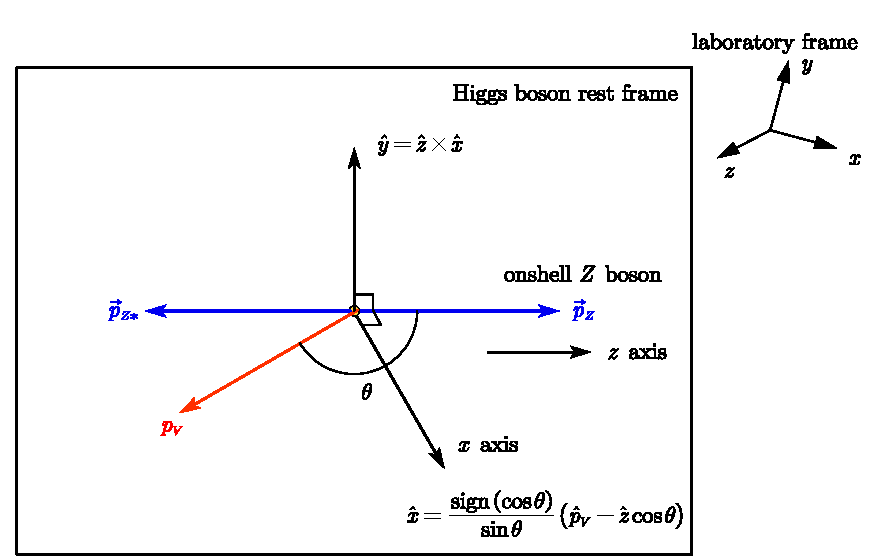
\includegraphics[width=0.5\textwidth]{figure/referenceSystem.pdf}%Path of the figure%
%     \caption{Reference System in 3-dim }%Title of the figure%
%     \label{fig:ref3d}
% \end{figure}
\subsection{Density matrix and observable quantity}
Defining the z-axis as the direction of on-shell Z boson's 3-momentum, we can choose \(J_z\) as the polarization operator and eigenstates of \(J_z\) as the basis of the spin space. In our case with two spin-1 massive bosons' system (i.e., two-qutrit system), both Z bosons are from Higgs decay, and the spin component is conserved in the CM frame. Therefore, the ZZ state can only lie in one of 3 joint states, i.e., \({\ket{l_1l_2}\in\{\ket{-+}, \ket{00}, \ket{+-}}\}\), where \(l_1\) and \(l_2\) are the spin states of two Z bosons. In quantum mechanics, the density matrix is a useful tool to describe the state of a quantum system. By definition, the density matrix of a two-qutrit ZZ system can be written as a tensor production
\begin{align}
    \rho=\sum p_{l_1l_2}\ket{l_1l_2}\bra{l_1l_2},
\end{align} 
where \(p_{l_1l_2}\) is the possibility on \(\ket{l_1l_2}\), and \(p_{l_1l_2}\geq1,\quad\sum p_{l_1l_2}=1\)~\cite{Aguilar-Saavedra:2022wam}.   
 
  \begin{figure}[htb]     
    \centering
     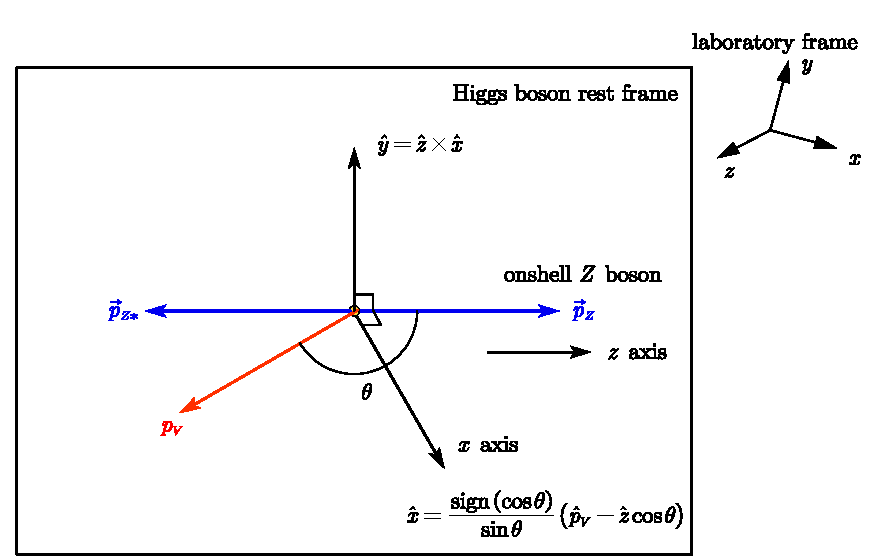
\includegraphics[width=0.45\textwidth]{figure/figure0_reference.pdf}%Path of the figure%
     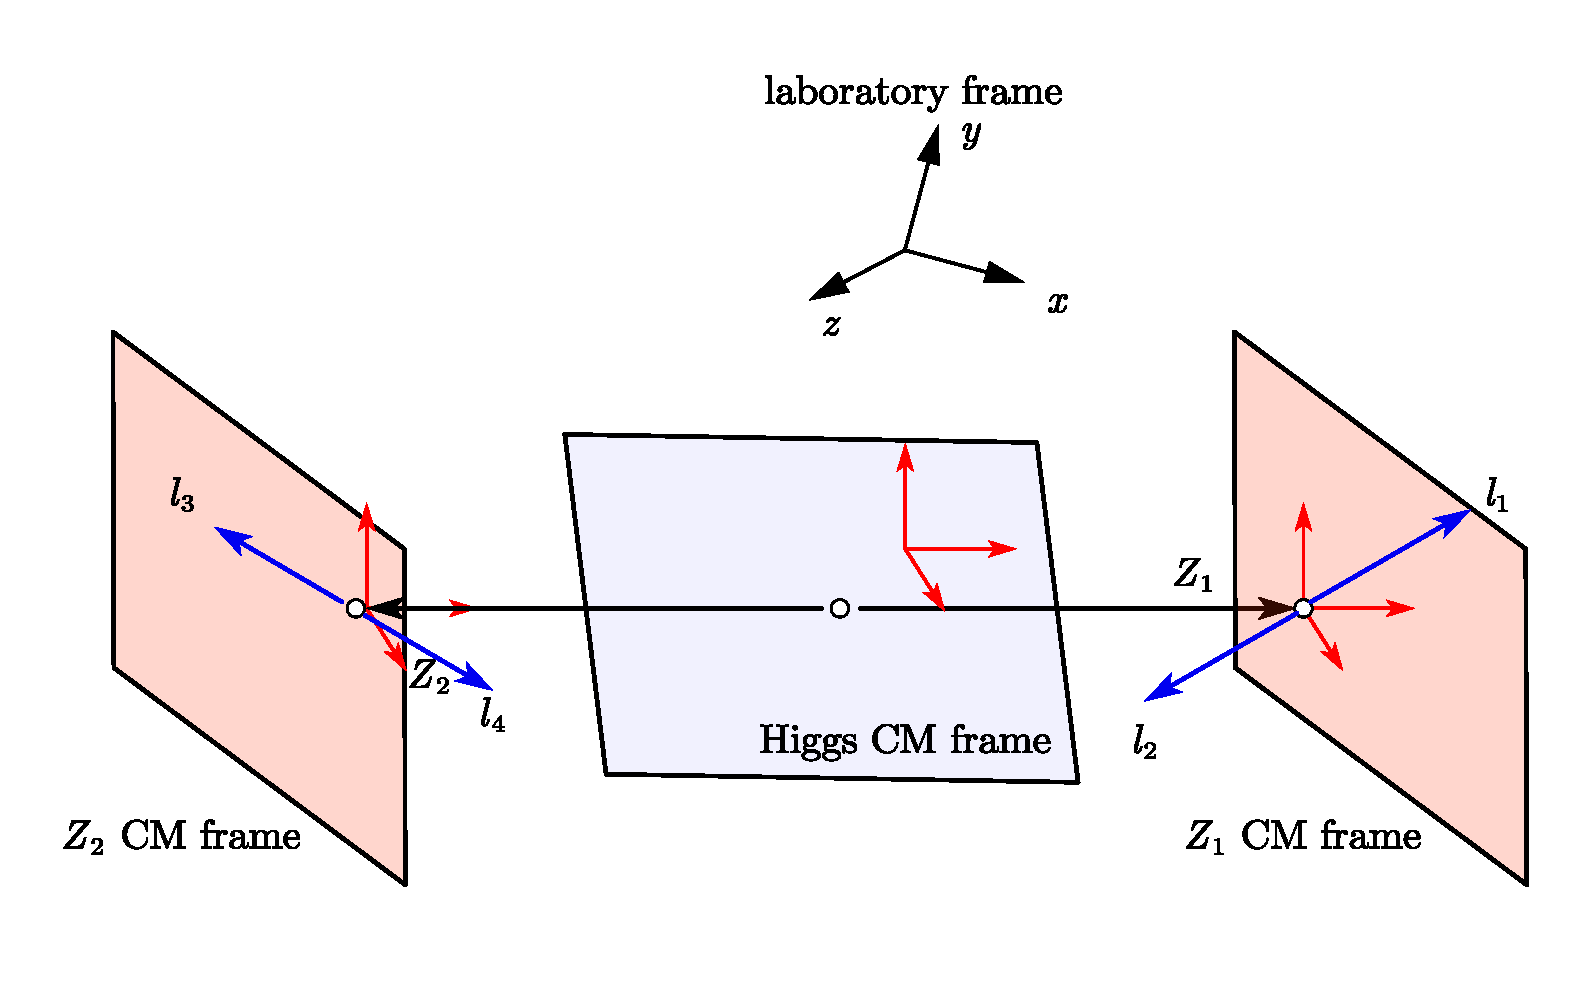
\includegraphics[width=0.45\textwidth]{figure/figure0_frame.pdf}%Path of the figure%
     \caption{Definition of Reference System. In Higgs CM frame, we define on-shell bosons as z-axis so that we create coordinate. In the lepton CM frame, we will still use this coordinate system for the direction angles of the leptons. }%Title of the figure%
     \label{fig:frame}
 \end{figure}
 
For more general case, we can construct the wave vector \(\varepsilon^\mu(p,\lambda)\), which is the polarization vector of a spin-1 particle with momentum \(p\) and helicity \(\lambda\). In our case, we choose Minkowski metric \(g_{\mu\nu}=\mathrm{diag}(1,-1,-1,-1) \). For the benefit of the relative simplicity of our expression, we first boost the Z boson to the CM frame of the Higgs boson. Then we determine z-axis which z unitary vector \(\hat{k}\) as the direction of the on-shell Z boson, and determine XOZ plane which contains \(\hat{k}\) and unit vector \(\hat{x}\) in laboratory frame, so that we can write x-axis unit vector \(\hat{r}=\mathrm{sign}(\cos\Theta)(\hat{x}-\hat{k}\cos\Theta)/\sin\Theta\). At present, we have constructed the z-axis and x-axis unit vectors and easily get y-axis $\hat{n}=\hat{k}\times\hat{r}$ to obtain a 3 dim reference system frame as figure \ref{fig:frame}. On this basis, we will construct the boosted basis vector in the lepton CM frame according to the coordinate system of the 3-dim. The boosted basis vector can be expressed as
\begin{align}
    n_1^\mu(1)=n_1^\mu(2)=(0,\hat{n}), ~~~
    n_2^\mu(1)=n_2^\mu(2)=(0,\hat{r}), ~~~
    n_3^\mu(1)=\gamma(\beta,\hat{k}),~~~
    n_3^\mu(2)=\gamma(-\beta,\hat{k}),
\end{align}
where \(-\beta, \gamma\) is CM frame Lorentz boost parameters, and the indices \(1,2\) represent the two Z bosons. The polarization vector can be written by the representation of eigenstates of \(S_3\) as
\begin{align}
    \varepsilon^\mu(p,\lambda)=\frac{1}{\sqrt{2}}|\lambda|(\lambda n_1^\mu+\mathrm{i}n_2^\mu)+(1-|\lambda|)n_3^\mu.
    \label{eq:polarization}
\end{align} 
%For one Z boson, this state vector is the all possible polarization states \(\varepsilon^\mu(p,\lambda)\) of the Z boson in different helicity \(\lambda\), each of which has a corresponding probability amplitude \(\mathcal{M(\lambda)}\) (the probability a \(p\) momentum \(Z\) boson has \(\lambda\) helicity). 
The probability amplitude of the \(ZZ\) process is then formulated as
\begin{align}
    \mathcal{M} \left( \lambda _1,\lambda _2 \right) =\mathcal{M} _{\mu \nu}\varepsilon ^{\mu}\left( p_1,\lambda _1 \right) \varepsilon ^{\nu}\left( p_2,\lambda _2 \right),
    \label{eq:amplitude} 
\end{align}
which is the probability amplitude for \(Z_1\) with momentum \(p_1\) and helicity \(\lambda_1\), and \(Z_2\) with momentum \(p_2\) and helicity \(\lambda_2\). 
By the definition of the density matrix, in general, the density matrix of the two-qutrit system can be written as \(\rho=\sum p_{ll'}\ket{l}\bra{l'}\) . According to the discussion above, while \(\ket{l}\) is the state function of the two \(Z\) bosons, this joint state function is actually 
\begin{align}
    \ket{\Phi}=\sum c_{ij} \ket{ij}\longrightarrow\sum \mathcal{M}(\lambda_1,\lambda_2)\ket{\lambda_1,\lambda_2},
\end{align}
where \(c_{ij}\) is the coefficient of the joint state function. 
Therefore, the density matrix components is
\begin{align}
    \rho=\ket{\Phi}\bra{\Phi}\rightarrow\rho_{iji'j'}&=c_{ij}c_{i'j'}^*\\
    &=\frac{1}{|\bar{\mathcal{M}}|^2}\mathcal{M}(\lambda_1,\lambda_2)\mathcal{M}(\lambda_1',\lambda_2')^*.
\end{align}
Now we can represent density matrix components by probability amplitude defined in Eq.~\ref{eq:amplitude} as
\begin{align}
    \rho \left( \lambda _1,\lambda _{1}^{\prime},\lambda _2,\lambda _{2}^{\prime} \right) =\frac{\mathcal{M}(\lambda_1,\lambda_2)\mathcal{M}(\lambda_1',\lambda_2')}{|\bar{\mathcal{M}}|^2}= \frac{1}{|\bar{\mathcal{M}}|^2} \left( \mathcal{M} _{\mu \nu}\varepsilon ^{\mu}\left( p_1,\lambda _1 \right) \varepsilon ^{\nu}\left( p_2,\lambda _2 \right) \right) \left( \mathcal{M} _{\mu' \nu'}\varepsilon ^{\mu'}\left( p_1,\lambda _1' \right) \varepsilon ^{\nu'}\left( p_2,\lambda _2' \right) \right) ^{\dag}.
\end{align}
Here \(\bar{\mathcal{M}}\) is the normalization factor of the probability amplitude. Moreover, we can construct the covariance helicity projector operator \(\mathscr{P}_{\lambda\lambda'}^{\mu\nu}\)from Eq.~\ref{eq:polarization} in the lepton CM frame boosted by momentum \(p\), which can be defined as
\begin{align}
    \mathscr{P} _{\lambda \lambda '}^{\mu \nu}\left( p \right) &=\varepsilon ^{\mu}\left( p,\lambda \right) \varepsilon ^{\nu}\left( p,\lambda' \right).
\end{align}
Using the covariance helicity projector operator, the density matrix can be simplified as 
\begin{align}
    \rho \left( \lambda _1,\lambda _{1}^{\prime},\lambda _2,\lambda _{2}^{\prime} \right) =\frac{\mathcal{M} _{\mu \nu}\mathcal{M} _{\mu \prime\nu \prime}^{\dagger}\mathscr{P} _{\lambda _1\lambda _{1}^{\prime}}^{\mu \mu \prime}\left( p_1 \right) \mathscr{P} _{\lambda _1\lambda _{1}^{\prime}}^{\mu \mu \prime}\left( p_2 \right)}{|\bar{\mathcal{M}}|^2}.
\end{align}
%  \textcolor{red}{\large Some narrative may be added here for the quantum mechanical definition of the density matrix using the state function of the $ZZ$ states. Please also explain the form of the ZZ function with the above polarization vector.}
% ok @youpeng
 The form of the density matrix describing the polarization state of the two-qutrit system formed by two spin-1 bosons can generally be parameterized using Gell-Mann matrices ~\cite{Fabbrichesi:2023cev,Barr:2024djo} 
\begin{align}
\rho(\lambdaA,\lambdaAp,\lambdaB,\lambdaBp)= \Big(\frac{1}{9}\left[\mathbb{1}_3\otimes
    \mathbb{1}_3\right]+
    \sum_a f_a \left[T^a\otimes \mathbb{1}_3\right]+\sum_a g_a \left[\mathbb{1}_3\otimes T^a\right] 
    +\sum_{ab} h_{ab}  \left[T^a\otimes T^b\right]\Big)_{\lambdaA\lambdaAp\lambdaB\lambdaBp},
    \label{eq:rho1}
\end{align}
where $T^a$, $T^b$ are the $3\times
3$ Gell-Mann matrices with $a=1,2,\dots, 8$. The coefficients $f_a$ and $g_a$  are components of the spin polarization vector, and $h_{ab}$ being correlation coefficients for \(ZZ\) system. In this way, we will have 80 parameters to be determined from observed data. Applications of this method to probe quantum entanglement can be found in the papers~\cite{Fabbrichesi:2023cev,Barr:2024djo}
Using Gell-Mann matrices to represent the density matrix~\ref{eq:rho1} is one of the possible parameterization. There is another simple yet effective way to parameterize the density matrix by using irreducible tensor operators~\cite{Aguilar-Saavedra:2015yza, Aguilar-Saavedra:2017zkn, Rahaman:2021fcz}
\begin{equation}
    \rho = \frac19\left[
    \II_3\otimes\II_3 + A_{LM}^1 T_{M}^L\otimes\II_3 + A^2_{LM}\II_3\otimes T^L_{M} + C_{L_1M_1L_2M_2}T^{L_1}_{M_1}\otimes T_{M_2}^{L_2}
    \right],
    \label{eq:rho2}
\end{equation}
where $T^L_M$ are the irreducible tensor operators complying with a trace rule such that ${\rm Tr}\left[T_{M}^L (T^L_M)^\dagger\right]$ = 3. It should be noted that a sum over the indices $L = 1, 2$ and $-L \leq M \leq L $. These tensor operators are usually expressed as linear combination of the spin spin operators for spin-1 particles. One may refer to paper~\cite{Aguilar-Saavedra:2022wam} for the exact form of these operators. The coefficients $A^i_{LM}$ and $C_{L_1M_1L_2M_2}$ are similar to the ones in Eq.~\ref{eq:rho1} representing both  the polarizations and spin correlations. In both parametrization form, we may extract the corresponding coefficients from simulated or actual data, which is very challenging because both the CM frame of the colliding beam and the rest frame of the decaying particles should be established correctly so that the angular distributions of the final lepton can be determined precisely. Consequently, there will be multiple Lorentz boost or transformation between coordinate systems.  However, in the tensor-parametrization form of the density matrix, the number of parameters to be determined reduces to three parameters.
In order to extract the coefficients of the density matrix, a relation between these coefficients and a direct observable in the experiment is needed. This has been done through a quantum state tomography for weak decays of massive bosons~\cite{Ashby-Pickering:2022umy}. The high energy collider experiments directly provide the general observable quantity, cross section, which can be expressed in terms of decaying matrix density of the massive bosons. For example, the differential cross section fro $ZZ\to \ell_1^+\ell_1^-\ell_2^+\ell_2^-$ can be written~\cite{Rahaman:2021fcz}
\begin{equation}
    \frac{1}{\sigma} \frac{d\sigma}{d\Omega_+ \, d\Omega_-} = \left( \frac{3}{4\pi} \right)^2 \mathrm{Tr} \left[ \rho_{V_1 V_2} \left( \Gamma_1 \otimes \Gamma_2 \right) \right],
    \label{eq:xsection}
\end{equation}
where the solid angles $d\Omega^{\pm} \sin\theta^{\pm}d\theta^{\pm}d\phi^{\pm}$ are given in terms of the spherical coordinates for the momenta of the final charged leptons with respect to the rest frame of the decaying Z boson. $\rho_{V_1V_2}$ is the density matrix for the entangled $ZZ$ state. The decaying density matrix of a Z boson into charged leptons is given as~\cite{Rahaman:2021fcz,Aguilar-Saavedra:2022wam,Aguilar-Saavedra:2022mpg}
\begin{equation}
\Gamma(\theta, \phi) = \frac{1}{4} 
\begin{pmatrix}
1 + \cos^2 \theta - 2 \eta_\ell \cos \theta & \frac{1}{\sqrt{2}} (\sin 2\theta - 2\eta_\ell \sin \theta)e^{i\phi} & (1 - \cos^2 \theta)e^{i2\phi} \\
\frac{1}{\sqrt{2}} (\sin 2\theta - 2\eta_\ell \sin \theta)e^{-i\phi} & 2 \sin^2 \theta & -\frac{1}{\sqrt{2}} (\sin 2\theta + 2\eta_\ell \sin \theta)e^{i\phi} \\
(1 - \cos^2 \theta)e^{-i2\phi} & -\frac{1}{\sqrt{2}} (\sin 2\theta + 2\eta_\ell \sin \theta)e^{-i\phi} & 1 + \cos^2 \theta - 2 \eta_\ell \cos \theta
\end{pmatrix},
\end{equation}
where the spherical coordinates $\theta$ and $\phi$ are the angles of the three momentum of the negative  charged lepton in the $Z$ boson rest frame. The trace can be simplified further using the normalization property of the irreducible tensors and making use of spherical harmonic functions $Y_L^M(\theta, \phi)$ so that Eq.~\ref{eq:xsection} can be written in the following form:
\begin{align}
    \frac{1}{\sigma}\frac{d\sigma}{d\Omega_1d\Omega_2} =&\frac{1}{(4\pi)^2} [ 1+A_{LM}^1Y_L^M(\theta_1,\phi_1)+A_{LM}^2B_LY_L^M(\theta_2,\phi_2)\\
    & +C_{L_1M_1L_2M_2}B_{L_1}B_{L_2}Y_{L_1}^{M_1}(\theta_1,\phi_1)Y_{L_2}^{M_2}(\theta_2,\phi_2)
    ] ,
\end{align}
with $B_1 = -\sqrt{2\pi}\eta_{\ell}$, and $B_2 = \sqrt{2\pi/5}$.

Now the coefficients in Eq.~\ref{eq:rho2} can be expressed using the above differential cross section making use of orthogonal property of the spherical harmonics:
\begin{align}
    \int \frac{1}{\sigma}\frac{d\sigma}{d\Omega_1d\Omega_2}Y_L^M(\Omega_j)d\Omega_j&=\frac{B_L}{4\pi}A_{LM}^j, \qquad j=1,2;\\
    \int \frac{1}{\sigma}\frac{d\sigma}{d\Omega_1d\Omega_2}Y_{L_1}^{M_1}(\Omega_1)Y_{L_2}^{M_2}(\Omega_1)d\Omega_1d\Omega_2 &= \frac{B_{L_1}B_{L_2}}{4\pi}C_{L_1M_1L_2M_2}.
\end{align}

It is worth noting that the $ZZ$ system is in the singlet state because the third component of the spin along the boson momentum direction is conserved. This imposes strong constraints on the density matrix, including only nine non-zero elements with the relation
\begin{equation}
    C_{2,2,2,-2} = \frac{1}{\sqrt{2}}A_{2, 0}^1.
\end{equation}

\subsection{CHSH inequality derivation}

The proof\cite{clauser1974experimental} of the CHSH inequality is based on the following assumptions: \textbf{Local hidden variable} theories: the measurement results of the two particles are determined by the hidden variables of the particles themselves, and the measurement results of the two particles are independent of each other.

We assume there a pair of entangled particles for \(a\), \(a^\prime\), \(b\), \(b^\prime\) are different measurement directions, and \(A\), \(A^\prime\), \(B\), \(B^\prime\) are the measurement results which's possibe value are \(\{-1,0,1\}\). In other words, \(A\) are observables in \(\mathcal{H}_A\), and \(B\) are observables in \(\mathcal{H}_B\). If the local hidden variable theories are correct, the possiblity of pairs of outcomes \(P(a,b)\) is: 
\[P(a,b)=\int d\lambda A(a,\lambda) B(b,\lambda) \rho(\lambda) \]
where \(\lambda\) is the hidden variable, and \(\rho(\lambda)\) is the probability distribution of the hidden variable. So that:
\begin{align*}
    &P(a,b)-P(a,b^\prime)\\
    &=\int d\lambda \rho(\lambda) [A(a,\lambda)B(b,\lambda)-A(a,\lambda)B(b^\prime,\lambda)]\\
    &=\int d\lambda \rho(\lambda) [A(a,\lambda)B(b,\lambda)-A(a,\lambda)B(b^\prime,\lambda)\pm A(a,\lambda)B(b^\prime,\lambda)A(a^\prime,\lambda)B(b^\prime,\lambda)\mp A(a,\lambda)B(b^\prime,\lambda)A(a^\prime,\lambda)B(b^\prime,\lambda) ] \\
    &=\int d\lambda \rho(\lambda) A(a,\lambda) B(b,\lambda)[1\pm A(a^\prime,\lambda)B(b^\prime,\lambda)]-A(a,\lambda)B(b^\prime,\lambda)[1\pm A(a^\prime,\lambda)B(b,\lambda)]
\end{align*}
apply the triangle inequality  (\(c=a+b\Rightarrow|c|\leqslant |a|+|b|\)):
\begin{align*}
    &|P(a,b)-P(a,b^\prime)|\\
    &\leqslant \left|\int d\lambda \rho(\lambda) A(a,\lambda) B(b,\lambda)[1\pm A(a^\prime,\lambda)B(b^\prime,\lambda)]\right|+\left|\int d\lambda \rho(\lambda) A(a,\lambda)B(b^\prime,\lambda)[1\pm A(a^\prime,\lambda)B(b,\lambda)]\right|\\
    &\leqslant \int d\lambda \left|A(a,\lambda) B(b,\lambda)\right|\left|1\pm A(a^\prime,\lambda)B(b^\prime,\lambda)\right|+\int d\lambda \left|A(a,\lambda)B(b^\prime,\lambda)\right|\left|1\pm A(a^\prime,\lambda)B(b,\lambda)\right|\\
\end{align*}
cause \([1\pm A(a^\prime,\lambda)B(b^\prime,\lambda)]\rho(\lambda) \geqslant 0 \), and \([1\pm A(a^\prime,\lambda)B(b,\lambda)]\rho(\lambda) \geqslant 0 \) they are \textbf{non-negative}. \marginpar{Because both A, B, A', B' are \(\{-1,0,1\}\), the absolute value of the product of them is 1.} Then we have:
\begin{align*}
    &|P(a,b)-P(a,b^\prime)|\\
    &\leqslant \int d\lambda \rho(\lambda) [1\pm A(a^\prime,\lambda)B(b^\prime,\lambda)]+\int d\lambda \rho(\lambda) [1\pm A(a^\prime,\lambda)B(b,\lambda)]\\
    &\leqslant 2 \pm \left[\int d\lambda \rho(\lambda) A(a^\prime,\lambda)B(b^\prime,\lambda) + \int d\lambda \rho(\lambda) A(a^\prime,\lambda)B(b,\lambda)\right]\\
    &\leqslant 2 \pm \left[P(a^\prime,b^\prime)+P(a^\prime,b)\right]
\end{align*}
where the last inequality is the definition of \(P(a^\prime,b^\prime)\) and \(P(a^\prime,b)\). So that\marginpar{We use triangle inequality again}:
\begin{align*}
    &|P(a,b)-P(a,b^\prime)|\leqslant 2 \pm \left[P(a^\prime,b^\prime)+P(a^\prime,b)\right]\\
    &\Rightarrow |P(a,b)-P(a,b^\prime)|+|P(a,b)+P(a,b^\prime)|\leqslant 2\\
    &\Rightarrow |P(a,b)-P(a,b^\prime)+P(a,b)+P(a,b^\prime)|\leqslant \text{Left.} \leqslant 2
\end{align*}
Q.E.D. 

But for the quantum mechanics, the measurement results of the two particles are not independent of each other, so that the CHSH inequality is violated. for two particles with spin \(1\), the state of particles is: \(\{\ket{+},\ket{0},\ket{-}\}\), so pair of particles are in the state:
\[\{\ket{+},\ket{0},\ket{-}\}_A\otimes\{\ket{+},\ket{0},\ket{-}\}_B\]
Cause limit of spin momentum conservation, the state of the two particles must be:
\[\ket{\psi_{s}}=\frac{1}{\sqrt{3}}(\ket{+-}-\ket{00}+\ket{-+})\]


\subsection{CGLMP inequality}
Our measurement is based on 3 dimension (spin 1)In Spin-1 case (3 dimension), the density matrix\marginpar{Detiel of proof in ~\cite{fabbrichesi_bell_2023} section 2.3}
%[TODO] add density matrix of spin 1

For pherhaps of local hidden variable theories, CGLMP inequality\cite{dalton2021cglmp}, in the case of two particles with spin \(1\), the inequality\cite{Collins_2002} is:
\begin{align*}
    I_3\leq &2 \\
    \textrm{which:}\quad I_3 = &+[P(A_1=B_1)+P(B_1=A_2+1)\\
          &+P(A_2=B_2)+P(B_2=A_1)]\\
          &-[P(A_1=B_1-1)+P(B_1=A_2)\\
          &+P(A_2=B_2-1)+P(B_2=A_1-1)]
\end{align*}
where \(A_i\) and \(B_i\) are the measurement results of the two particles, and \(P(A_i=B_j)\) is the probability of the two particles having the same measurement results. We can use Bell operator \(\mathcal{O}_{Bell}\) for the inequality:
\[I_3=\braket{\mathcal{O}_{Bell}}=\mathrm{tr}\{\rho \mathcal{O}_{Bell} \}\leqslant 2\]

For our \(H\rightarrow ZZ\) process, \(ZZ\) state must be:
\[\ket{\psi_{ZZ}}=a_1\ket{+-}+a_2\ket{00}+a_3\ket{-+}\]
where \(a_1^2+a_2^2+a_3^2=1\). 
\[e_\sigma^\mu(m,\vec{k})=\begin{array}{c:c}
	\,\, &		{\color[RGB]{0,0,255}\begin{matrix}
	S_-&	\quad S_0&		\quad S_0\\
\end{matrix}}\\\hdashline{\color[RGB]{0, 0, 255} \begin{array}{c}k_0\\k_x\\k_y\\k_z\\
\end{array}}&		\left[ \begin{matrix}0&		\frac{|\vec{k}|}{m}&		0\\-\frac{1}{\sqrt{2}}&		0&		\frac{1}{\sqrt{2}}\\\frac{i }{\sqrt{2}}&		0&		\frac{i}{\sqrt{2}}\\0&		-\frac{\sqrt{k^2}}{m}&		0\\
\end{matrix} \right]\\
\end{array}\]
\[\ket{\psi_{ZZ}}=\eta_{\mu\nu}e_\sigma^\mu(m_1,\vec{k})e_\lambda^\nu(m_2,-\vec{k})\ket{\vec{k},\sigma}_A\ket{-\vec{k},\lambda}_B \]

this time, the \(\psi\) can be written in Spin-1 basis:
\[\psi=(0,0,1,0,-\beta,0,1,0,0)\]
and the density matrix is tensor product of the state:
\[
    \begin{bmatrix}
     0 & 0 & 0 & 0 & 0 & 0 & 0 & 0 & 0 \\
     0 & 0 & 0 & 0 & 0 & 0 & 0 & 0 & 0 \\
     0 & 0 & 1 & 0 & -\beta  & 0 & 1 & 0 & 0 \\
     0 & 0 & 0 & 0 & 0 & 0 & 0 & 0 & 0 \\
     0 & 0 & -\beta  & 0 & \beta ^2 & 0 & -\beta  & 0 & 0 \\
     0 & 0 & 0 & 0 & 0 & 0 & 0 & 0 & 0 \\
     0 & 0 & 1 & 0 & -\beta  & 0 & 1 & 0 & 0 \\
     0 & 0 & 0 & 0 & 0 & 0 & 0 & 0 & 0 \\
     0 & 0 & 0 & 0 & 0 & 0 & 0 & 0 & 0 \\
    \end{bmatrix}
\]



% \section{Simulation results}

% now we have the following results:

% \begin{table}[htb]
%     \caption{Simulation results}
%     \label{tab:simres}
%     \centering
%     \begin{tabularx}{0.8\textwidth}{X|X|X|X|X}
%         \toprule
%         Energy & 0.0TeV & 10.0TeV & 20.0TeV & 30.0TeV \\
%         \midrule
%         I3 & - & \(2.5856307 \pm 1.3047833\) & - & - \\
%         \bottomrule
%     \end{tabularx}
% \end{table}
% \begin{figure}[htb]
%     \centering
%     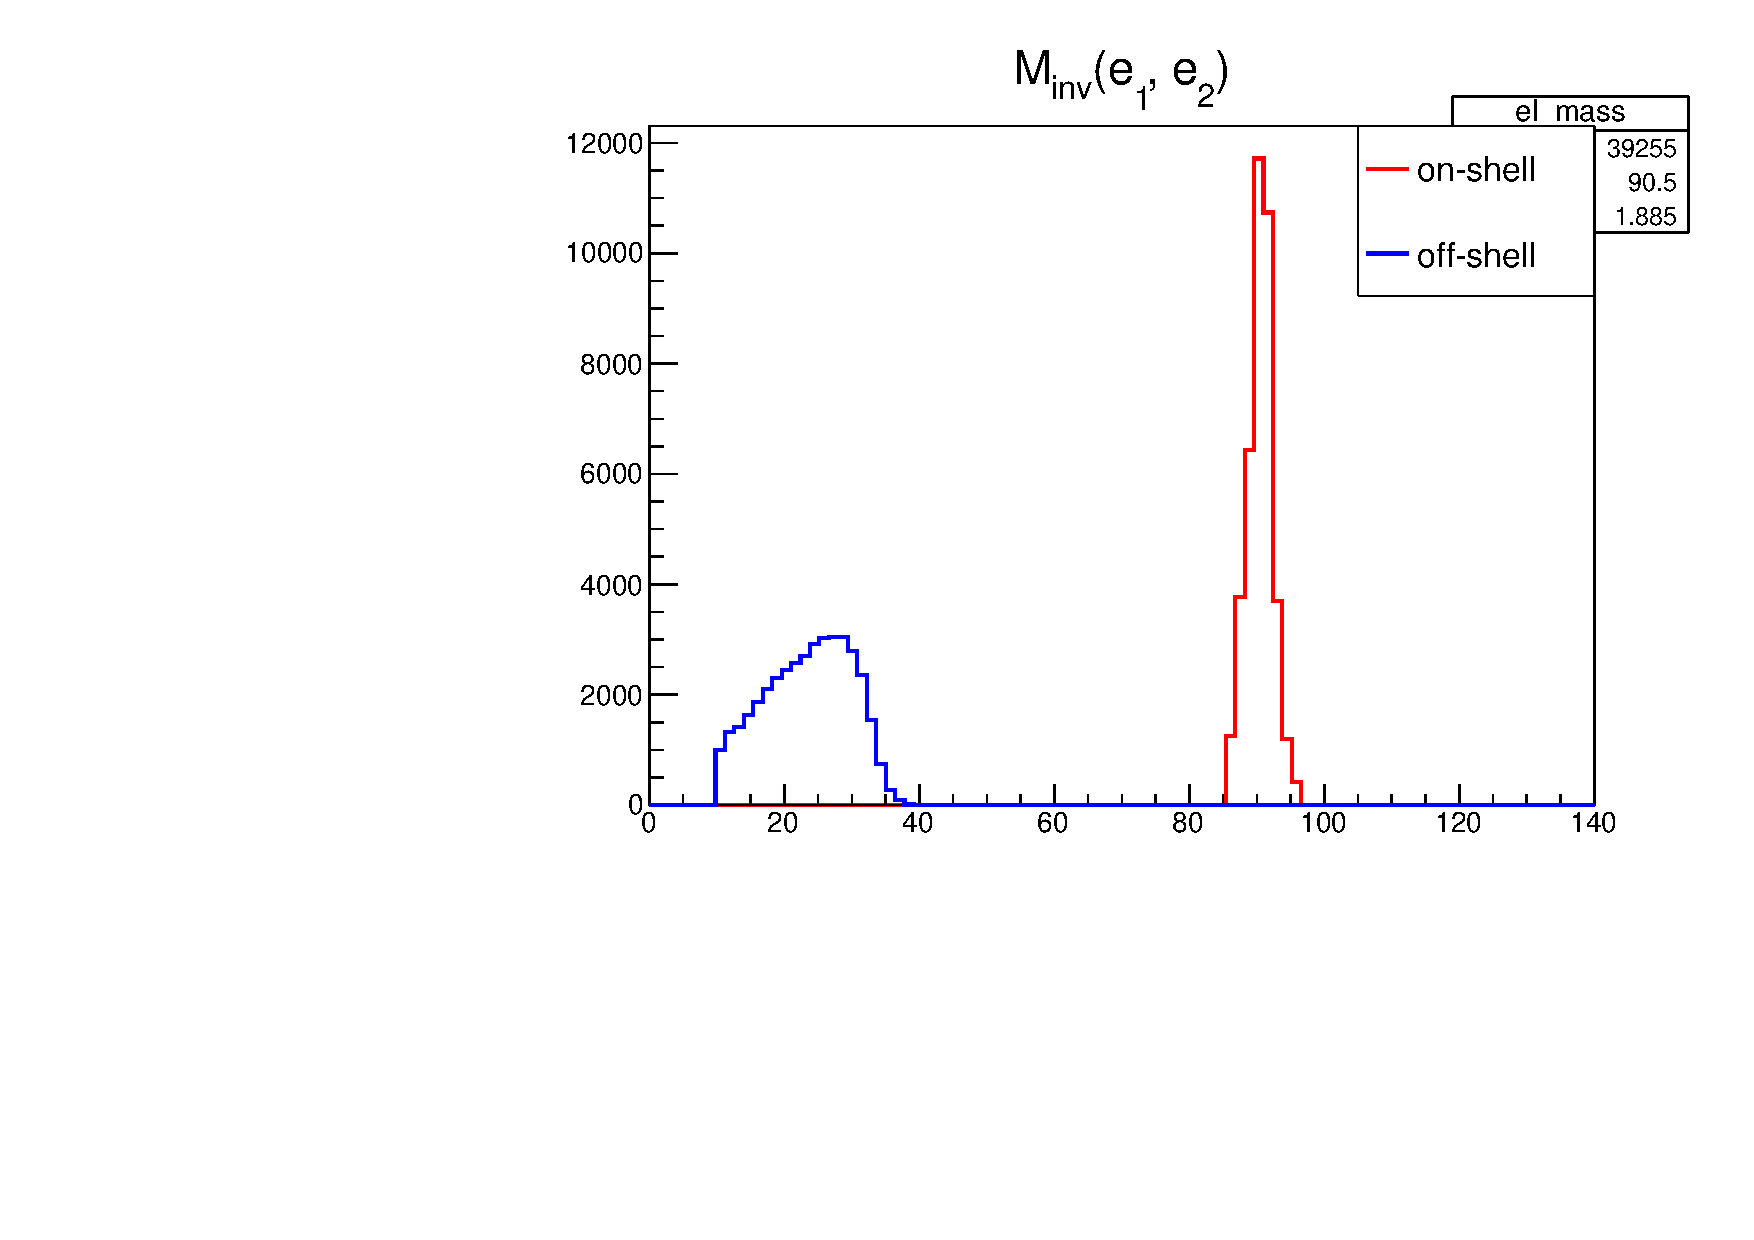
\includegraphics[width=0.7\textwidth]{figure/Mll_delphes.pdf}%Path of the figure%
%     \caption{Delphes Simulation}%Title of the figure%
%     \label{fig:mlldelphes}
% \end{figure}


\bibliographystyle{ieeetr}
\bibliography{refer}
\end{document}